% 图 2.1 —— 手工重建（四个面板 f / g / h / k）
%
% 做法：看图定「是什么」，算法在圈定区域内量「是多少」。
%
% ① 视觉清单（看图定）
%      f  两条轴 + 抛物线；阴影 = 抛物线上方 ∪ x 轴下方
%      g  同 f，只取竖轴右侧
%      h  两条轴 + 一条「先贴轴、再翘起」的曲线；阴影 = 曲线之上
%      k  同 h，只取竖轴右侧
%
% ② 区域内精测
%      画框   f x[18,260] y[51,392]   g x[317,557] y[51,388]
%             h x[622,860] y[51,239]  k x[920,1165] y[51,240]
%      轴     f/g (134|436, 236)      h (739,237)   k (1037,236)
%      抛物线 f：按「笔画比阴影线粗」（6px vs 3px）挑出两臂，58 个点最小二乘
%             → 顶点 (134,236)、**K = 0.0110**，纯抛物线即最优（残差中位 5.1px）
%      曲线 h/k：同法 → 比抛物线更贴轴，取 y = A·x² + C·x⁴（A=0.0080、C=1.0e-6）
%      阴影线 45°，间距 9.5
%
% ⚠ 两条做法要点（用户指出）：
%   1. 阴影**铺满整格**，曲线与轴画在上面。
%      （我一开始以为里面有个白 U 区、要用 clip 挖掉 —— 放大原图看，
%        阴影一直填到轴，U 里也有；判错方向。）
%   2. 曲线一律 `plot[domain]` **解析画**，不拿描摹点做样条 ——
%      描摹点带着扫描的纸张弯曲，串出来就是周期性波纹。
\documentclass[12pt]{standalone}
\usepackage{fontspec}
\setsansfont{Arial}
\newfontfamily\mfallback{DejaVu Sans}
\usepackage{tikz}
\usetikzlibrary{patterns}

\pgfdeclarepatternformonly{hatch45}
  {\pgfqpoint{-13.435pt}{-13.435pt}}
  {\pgfqpoint{13.435pt}{13.435pt}}
  {\pgfqpoint{13.435pt}{13.435pt}}
  {\pgfsetlinewidth{3.0pt}\pgfsetstrokecolor{black}%
   \pgfpathmoveto{\pgfqpoint{0pt}{0pt}}%
   \pgfpathlineto{\pgfqpoint{13.435pt}{13.435pt}}%
   \pgfusepath{stroke}}

\def\wAxis{5.0}
\def\wCurve{6.0}
\def\K{0.0110}          % f/g 的抛物线 y = 236 - K*(x-vx)^2
% \u26a0 f/g 也按 t∈[-1,1] 参数化：要画到 ±127 时 dx² 会到 16129pt，
%   超过 TeX 的维度上限 16383（实测 ±131 时 dx²=17161 就报 Dimension too large）。
\def\KF{330.64}         % = K·KDXF² = 0.0205 × 127²
\def\KDXF{127}

% h/k 的曲线：y = 237 − A·dx² − C·dx⁴，按 t = dx/KDX ∈[-1,1] 参数化，
% 常数吸收进 \qA \qB（直接用 dx 会让中间值到 1e8，TeX 报 Dimension too large）。
% ⚠ 宏名别用 \P —— TeX 内置 \P（¶），`\P2` 会被拆成 `\P`+`2`。
\def\KDX{94}        % 曲线出画框顶（y=51）处的 dx
\def\qA{86.77}          % = A·KDX² = 0.00982 × 8836
\def\qB{99.28}          % = C·KDX⁴ = 1.272e-6 × 78074896

\begin{document}
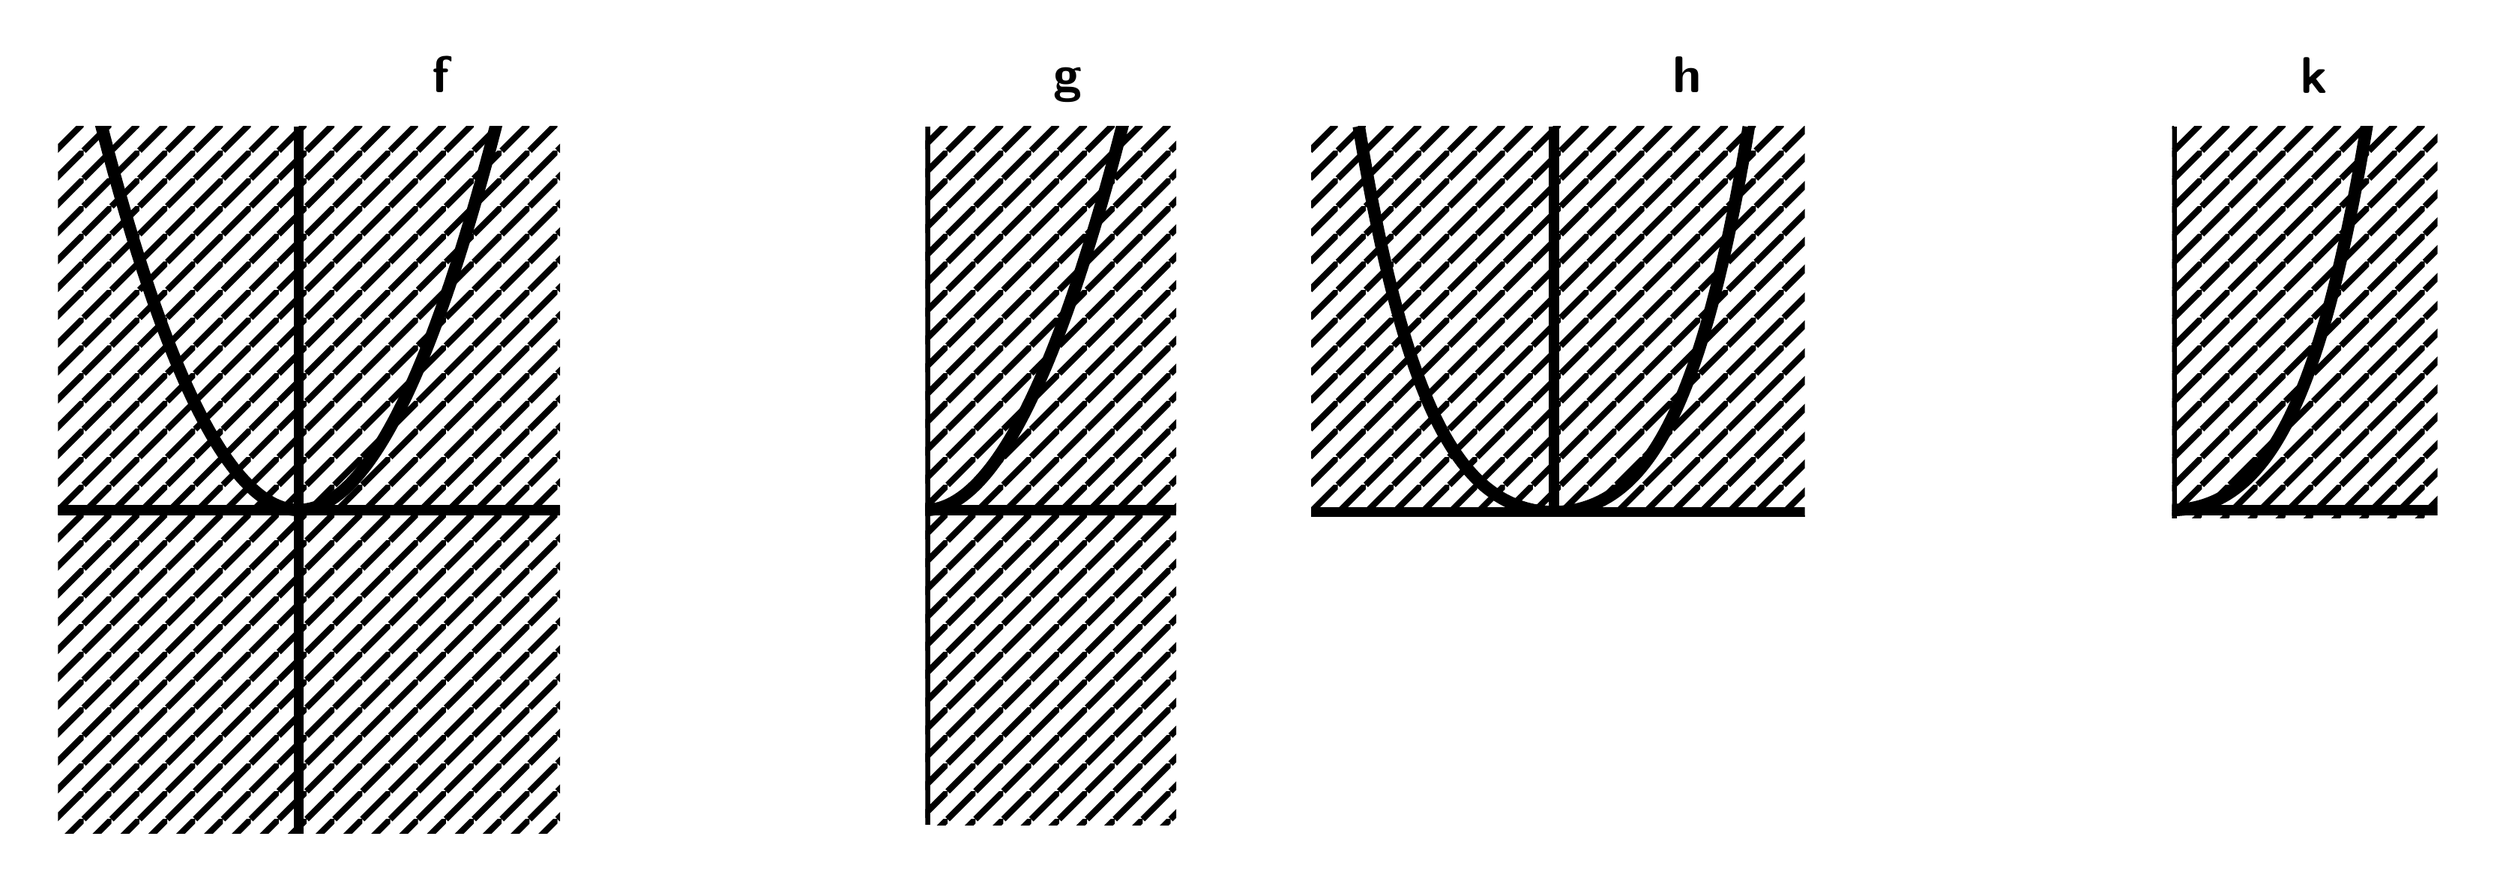
\begin{tikzpicture}[x=1pt, y=-1pt]

  % ════ f：面板 (18,51)-(260,392)，顶点 (134,236) ════
  \begin{scope}
    \clip (18,51) rectangle (260,392);
    \fill[pattern=hatch45] (18,51) rectangle (260,392);
    \draw[line width=\wAxis] (18,236) -- (260,236);
    \draw[line width=\wAxis] (134,51) -- (134,392);
    \draw[line width=\wCurve] plot[domain=-1:1,samples=181] (134+\KDXF*\x,{236-\KF*\x*\x});
  \end{scope}

  % ════ g：同 f，只取竖轴右侧 ════
  \begin{scope}
    \clip (436,51) rectangle (557,388);
    \fill[pattern=hatch45] (436,51) rectangle (557,388);
    \draw[line width=\wAxis] (317,236) -- (557,236);
    \draw[line width=\wAxis] (436,51) -- (436,388);
    \draw[line width=\wCurve] plot[domain=0:1,samples=121] (436+\KDXF*\x,{236-\KF*\x*\x});
  \end{scope}

  % ════ h：面板 (622,51)-(860,239)，顶点 (739,237) ════
  \begin{scope}
    \clip (622,51) rectangle (860,239);
    \fill[pattern=hatch45] (622,51) rectangle (860,239);
    \draw[line width=\wAxis] (622,237) -- (860,237);
    \draw[line width=\wAxis] (739,51) -- (739,239);
    \draw[line width=\wCurve] plot[domain=-1:1,samples=181]
         (739+\KDX*\x,{237-\qA*\x*\x-\qB*\x*\x*\x*\x});
  \end{scope}

  % ════ k：同 h 的曲线，平移到顶点 (1037,236)，只取右半 ════
  \begin{scope}
    \clip (1037,51) rectangle (1165,240);
    \fill[pattern=hatch45] (1037,51) rectangle (1165,240);
    \draw[line width=\wAxis] (920,236) -- (1165,236);
    \draw[line width=\wAxis] (1037,51) -- (1037,240);
    \draw[line width=\wCurve] plot[domain=0:1,samples=121]
         (1037+\KDX*\x,{236-\qA*\x*\x-\qB*\x*\x*\x*\x});
  \end{scope}

  % ════ 标签（实测框中心；f/g/h/k 都是小写斜体）════
  \node[anchor=center,inner sep=1.5pt,fill=white,font=\fontsize{28}{35}\selectfont] at (203.5, 26.0) {\textsf{\textbf{\textit{f}}}};
  \node[anchor=center,inner sep=1.5pt,fill=white,font=\fontsize{28}{35}\selectfont] at (505.0, 31.0) {\textsf{\textbf{\textit{g}}}};
  \node[anchor=center,inner sep=1.5pt,fill=white,font=\fontsize{28}{35}\selectfont] at (803.5, 26.0) {\textsf{\textbf{\textit{h}}}};
  \node[anchor=center,inner sep=1.5pt,fill=white,font=\fontsize{28}{35}\selectfont] at (1105.5,26.5) {\textsf{\textbf{\textit{k}}}};

  % ⚠ 必须显式给 bounding box，否则 standalone 会按内容裁边，渲染尺寸就与图不一致
  \path[use as bounding box] (0,0) rectangle (1185,402);
\end{tikzpicture}
\end{document}
